\chapter{Architettura riusabile per backend di Protelis}
\section{Piattaforme di simulazione}
L'architettura utilizzata per Protelis si dimostra flessibile, adatta alla
portabilità su diversi sistemi reali\cite{Clark2015} e simulati quali
Alchemist\cite{alchemist} (Figura 3b) e NASA World Wind\cite{Bell2007}.

L'architettura utilizzata per Protelis si dimostra flessibile, adatta alla
portabilità su diverse piattaforme. Per fare ciò è necessario realizzare un
backend che definisca i meccanismi di comunicazione tra i dispositivi e
gestisca l'esecuzione della macchina virtuale Protelis.

% TODO: Descrizione di alchemist migliore
\subsection{Alchemist}
\begin{figure}
  \centering
  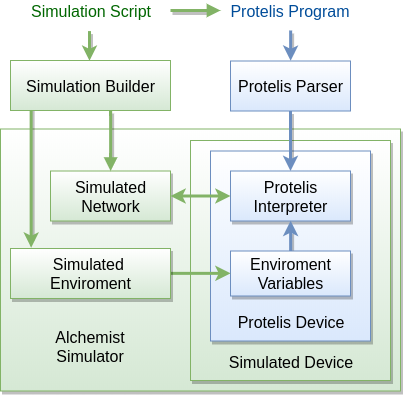
\includegraphics[width=0.7\linewidth]{images/alchemist-architecture.png}
  \caption{Implementazione di Protelis utilizzata in Alchemist.}
\end{figure}
Tra le realizzazioni esistenti l'esempio più rilevante è
Alchemist\footnote{https://alchemistsimulator.github.io/}: un simulatore per
computazione pervasiva, aggregata e ispirata alla natura. Esso utilizza al
proprio interno un meta-modello nel quale dispositivi vicini e interconnessi
comunicano seguendo un insieme di leggi ispirate al mondo della chimica.

Alchemist prevede la probabilità di utilizzare incarnazioni, ovvero
implementazioni concrete del proprio meta-modello per modellare uno specifico
concetto di interesse. Una di queste incarnazioni è quella che consente al
simulatore di eseguire un programma Protelis all'interno della propria
infrastruttura, che permette di creare e gestire una rete di nodi simulati
(Figura /ref{fig:alchemist-architettura}).

\subsection{NASA World Wind}
NASA World Wind\footnote{https://worldwind.arc.nasa.gov/} è un progetto
open-source cross-platform sviluppato dalla NASA, che offre un'interfaccia di
programmazione per creare, in maniera rapida, delle visualizzazioni 3D
interattive di un globo virtuale. Si differenzia da altri software simili come
Google Earth\footnote{https://www.google.it/intl/it/earth/} perché non è una
semplice applicazione, piuttosto un'intera SDK che può essere utilizzata come
base per costruire una propria applicazione.

È stato utilizzato per dimostrare come Protelis possa essere uno strumento che
permette di controllare anche dispositivi reali come uno sciame di droni. In
questa
simulazione\footnote{https://github.com/Protelis/Protelis-Demo-Visualized} 25
quadricotteri, disposti a griglia, volano a qualche centinaio di metri da
terra. Essi fanno uso di comunicazione a corto raggio, 500 metri, per parlare
con i dispositivi adiacenti.

\section{Sistemi distribuiti}

Un sistema distribuito è una collezione di computer indipendenti che appare
all'utente finale come un unico sistema coerente\cite{tanenbaum2016}.  Il
concetto di indipendenza implica che i dispositivi appartenenti al sistema non
abbiano risorse condivise, in particolare la memoria; allo stesso tempo questi
devono tenere un comportamento tra loro armonico. Deve essere quindi prevista
una modalità in cui questi componenti possano comunicare, per scambiarsi
informazioni e coordinarsi.

I costrutti fondanti della programmazione aggregata e i building block possono
semplificare notevolmente il design e lo sviluppo di applicazioni in un contesto
di Internet-of-Things\cite{DBLP:journals/computer/BealPV15}. Essa infatti
consente di costruire, tramite composizione delle proprie API, delle
applicazioni distribuite robuste e affidabili.

Al fine di eseguire macchine virtuali Protelis in un contesto distribuito è
necessario implementare un modello di scambio di messaggi tra queste (Figura
\ref{fig:distributed-deployment}).  L'architettura di Protelis (Sezione
\ref{subsec:Architettura di Protelis}) è stata ideata avendo questo problema ben
chiaro, pertanto è possibile estenderla facilmente, tramite l'implementazione di
uno strato middleware, che si occupi di ciò.


% TODO: API Protelis qui o in architettura?
\section{Architettura riusabile}
\label{sec:model-def}
L'obiettivo di questa sezione è di modellare una architettura del backend di
Protelis abbastanza flessibile, che consenta di incorporare la macchina virtuale
all'interno di un dispositivo, così che attraverso questo sia possibile
eseguirne le iterazioni. Concretamente si effettuerà un mapping delle
caratteristiche di un dispositivo (livello in basso nella Figura
\ref{fig:abstraction-layers}), così che queste possano essere utilizzate per
implementare i costrutti del \textit{field calculus}. Un obiettivo importante di
questo modello sarà circoscrivere in un'entità ben definita il concetto di
strategia di comunicazione. In questo modo il device sarà in grado di funzionare
indipendentemente dal metodo specifico scelto per realizzarla.

% TODO: da scrivere bene un'introduzione
\subsection{API di Protelis}
Le API del backend di Protelis sono scritte in Java, quindi sono facilmente
integrabili anche con linguaggi eseguiti sulla Java Virtual Machine. Esse
offrono le seguenti astrazioni.

\subsubsection{ExecutionContext}
Interfaccia che si pone fra una macchina virtuale Protelis e l'ambiente da cui
essa è circondata. I suoi compiti sono tre:
\begin{itemize}
\item tenere traccia dello stato persistente attraverso le iterazioni successive
  del prorgamma;
\item tenere traccia dell'ultimo stato condiviso dai dispositivi vicini;
\item tenere traccia dell'interazione del dispositivo con l'ambiente esterno
  (tempo, spazio, sensori, attuatori, ecc).
\end{itemize}

\subsubsection{ProtelisVM}
La macchina virtuale Protelis è il nucleo centrale dell'architettura: contiene
l'interprete del linguaggio che al proprio interno implementa gli operatori del
\textit{field calculus}. Accetta in input un \texttt{ProtelisProgram} e utilizza un
\texttt{ExecutionContext} per mantenere il proprio stato e interfacciarsi con
l'esterno. L'interfaccia permette di azionarne i cicli di esecuzione.

\begin{figure}
  \centering
  \includegraphics[width=\linewidth]{diagrams/output/protelis-api}
  \caption{Relazione tra \texttt{ProtelisVM}, \texttt{ExecutionContext} e
      \texttt{ProtelisProgram}.}
  \label{fig:uml-protelisvm}
\end{figure}

\subsubsection{AbstractExecutionContext}
L'interfaccia \texttt{ExecutionContext} contiene la definizione di molti metodi
che dovrebbero essere comuni a tutte le implementazioni di Protelis. Questa
entità astratta realizza quelle procedure delegando a una nuova entità, il
\texttt{NetworkManager}, il compito di stabilire un metodo efficace di
comunicazione.

\subsubsection{NetworkManager}
\label{sec:network-manager}
Astrazione di rete utilizzata dalla macchina virtuale Protelis: ad ogni
iterazione, la macchina virtuale ha bisogno di accedere all'ultimo stato
ricevuto dai vicini e di aggiornare lo stato che verrà inviato ad
essi. L'implementazione di questa interfaccia è cruciale, infatti definisce le
modalità di comunicazione tra i nodi della rete (Figura
\ref{fig:uml-protelisvm}).

Una considerazione importante da fare è che la documentazione ufficiale
specifica che non è necessario che lo stato venga ricevuto o inviato ad ogni
iterazione. La scelta della frequenza di aggiornamento dello stato è demandata
alla specifica implementazione di questa interfaccia, per trovare il rapporto
giusto tra efficienza e condivisione dello stato.

\begin{figure}
  \centering
  \includegraphics[width=\linewidth]{diagrams/output/networkmanager}
    \caption{Introduzione di \texttt{AbstractExecutionContext} e \texttt{NetworkManager}.}
  \label{fig:uml-networkmanager}
\end{figure}

\begin{figure}
  \centering
  \includegraphics[width=\linewidth]{diagrams/output/protelis-vm-sequence}
  \caption{Rappresentazione attraverso un diagramma di sequenza UML di un ciclo
    di esecuzione della macchina virtuale Protelis. Come si vede l'utilizzo di
    diversi \texttt{NetworkManager} specializza il comportamento di tutto il
    sistema.}
    \label{fig:uml-protelisvm-sequence}
\end{figure}


% TODO:
% Serializzazione:
% - time efficient
% - hashing (probabilità molto bassa di errore)
\subsubsection{CodePath}
Rappresenta un percorso, che parte dalla radice dell'albero di esecuzione della
macchina virtuale Protelis e termina in uno dei nodi. Supportando la
serializzazione, viene utilizzato per confrontare l'esecuzione locale a un nodo
con quella dei propri vicini e permettere l'allineamento del codice.

La specifica implementazione di questa classe è critica per la dimensione dei
pacchetti generati dalla comunicazione tra i nodi. Sarà necessario, quindi,
porre l'attenzione su questo aspetto quando la comunicazione sarà basata su
protocolli di rete.

All'interno delle API di Protelis sono già presenti due implementazioni di
questa interfaccia:
\begin{itemize}
\item \texttt{DefaultTimeEfficientCodePath}: il cui algoritmo di generazione è
  orientato alla velocità di esecuzione. L'output non è ottimizzato in termini
  di spazio. Questa implementazione non dovrebbe essere utilizzata quindi per
  l'utilizzo in una rete reale, perché potrebbe generare delle stringhe molto
  lunghe, con conseguenti problemi di performance;
\item \texttt{HashingCodePath}: il cui output dipende dall'algoritmo di hashing
  utilizzato. L'algoritmo di generazione è orientato all'ottimizzazione dello
  spazio, in quanto produce un output di lunghezza predicibile. Quindi è
  l'implementazione consigliata per l'utilizzo in una rete reale. Questa
  versione eredita dall'utilizzo delle funzioni di hashing il rischio di
  collisioni, che diminuisce con l'utilizzo di funzioni più complesse. Spetta al
  progettista la scelta della funzione di hashing che minimizzi le probabilità
  di collisione, massimizzando l'efficienza in termini computazionali.
\end{itemize}

\subsection{Definizione di nuovi concetti}
I concetti che seguono non fanno parte delle API di Protelis, ma sono stati
definiti appositamente per estenderle e creare quindi un nuovo modello, che sia
adatto a rappresentare dispositivi sia in un ambiente reale che in uno simulato.
Questo modello rappresenta dunque una possibile base di partenza per la
realizzazione di un backend di Protelis.

\subsubsection{Capacità di un dispositivo}
\label{sec:device-capabilities}

\begin{figure}
  \centering
  \includegraphics[width=\linewidth]{diagrams/output/device}
  \caption{Introduzione di \texttt{DeviceCapabilities} e \texttt{Device}.}
  \label{fig:uml-device}
\end{figure}

L'obiettivo di questa entità è di realizzare un \texttt{ExecutionContext},
traendo vantaggio delle funzioni già implementate in
\texttt{AbstractExecutionContext}. Implementa le seguenti caratteristiche di un dispositivo:
\begin{itemize}
\item \textbf{Mantenere uno stato nel tempo}: ovvero essere in grado di
  mantenere un insieme di variabili locali e aggiornarle in caso di necessità.
\item \textbf{Comunicare con altri dispositivi}: capacità e protocolli, regole
  utilizzate per effettuare uno scambio di informazioni con altri dispositivi
  vicini. Per fare questo viene riutilizzato il concetto di
  \texttt{NetworkManager} esistente in Protelis.
\item \textbf{Interagire con l'ambiente}: possibilità di interagire con il
  contesto da cui esso è circondato. In un contesto Internet-of-Things, per
  esemio, questo potrebbe concretizzarsi con l'utilizzo di sensori o attuatori.
\item \textbf{Eseguire funzioni definite dall'utente}: facoltà di definire
  funzioni, comportamenti che possono essere richiamate all'occorrente durante
  l'esecuzione del programma.
\end{itemize}

\subsubsection{Device}


Un \texttt{Device} (o dispositivo) è un concetto che rappresenta un singolo
dispositivo in una rete di nodi. Ciascuno di essi incorpora al proprio interno
una macchina virtuale Protelis e sfutta le proprie capacità
(\ref{sec:device-capabilities}), come l'interazione con l'ambiente esterno o la
capacità di mantenere lo stato di una variabile, per supportare l'esecuzione di
quest'ultima.

Un dispositivo per funzionare ha bisogno di un'implementazione concreta di
\texttt{NetworkManager} (\ref{sec:network-manager}), che viene specificata
durante la creazione di uno specifico oggetto, seguendo il pattern strategy. In questo modo il concetto di
dispositivo non è vincolato a uno specifico metodo di comunicazione. Nel
capitolo successivo è presente una dimostrazione della sua riusabilità.

\subsubsection{Speaker}
Implementato sotto forma di strategia funzionale, rappresenta la capacità di un
\texttt{Device} di pubblicare un messaggio, in un modo non definito dall'interfaccia, un
messaggio. Questo verrà gestito e utilizzato in modalità differenti, secondo
la strategia specificata.

La sua implementazione più elementare è \texttt{ConsoleSpeaker}, che prevede che
il messaggio venga stampato sullo standard output.
\begin{figure}
  \centering
  \subfloat[Deployment in simulatore]{
    \includegraphics[width=\linewidth]{diagrams/output/simulation-deployment}
    \label{fig:simulation-deployment}
  }\hfill
  \subfloat[Deployment in ambiente distribuito]{
    \includegraphics[width=\linewidth]{diagrams/output/distributed-deployment}
    \label{fig:distributed-deployment}
  }
  \caption{Rappresentazione attraverso un diagramma UML di deployment delle due
    differenti modalità di comunicazione utilizzate dal \texttt{NetworkManager}
    in contesti distribuiti e simulati. Nella prima i dispositivi appartengono a
    una memoria condivisa, possono usare questa per comunicare. Nella seconda
    ciascun dispositivo appartiene a una diversa Java Virtual Machine, quindi
    devono utilizzare un altro metodo per comunicare, per esempio le socket.}
\end{figure}